\section{Interval trees for orthogonal stabbing queries}
\label{sec:interval-trees}

In certain geometric applications like planar graphs, we might be interested in reporting the set of line segments $L$ associated with a window query  $w = [x_0, x_1] \times [y_0, y_1]$. 
%
This set $L$ contains all line segments with at least one end point inside $w$, or those segments that pass through the window $w$. 

\begin{figure}[ht!]
\centering
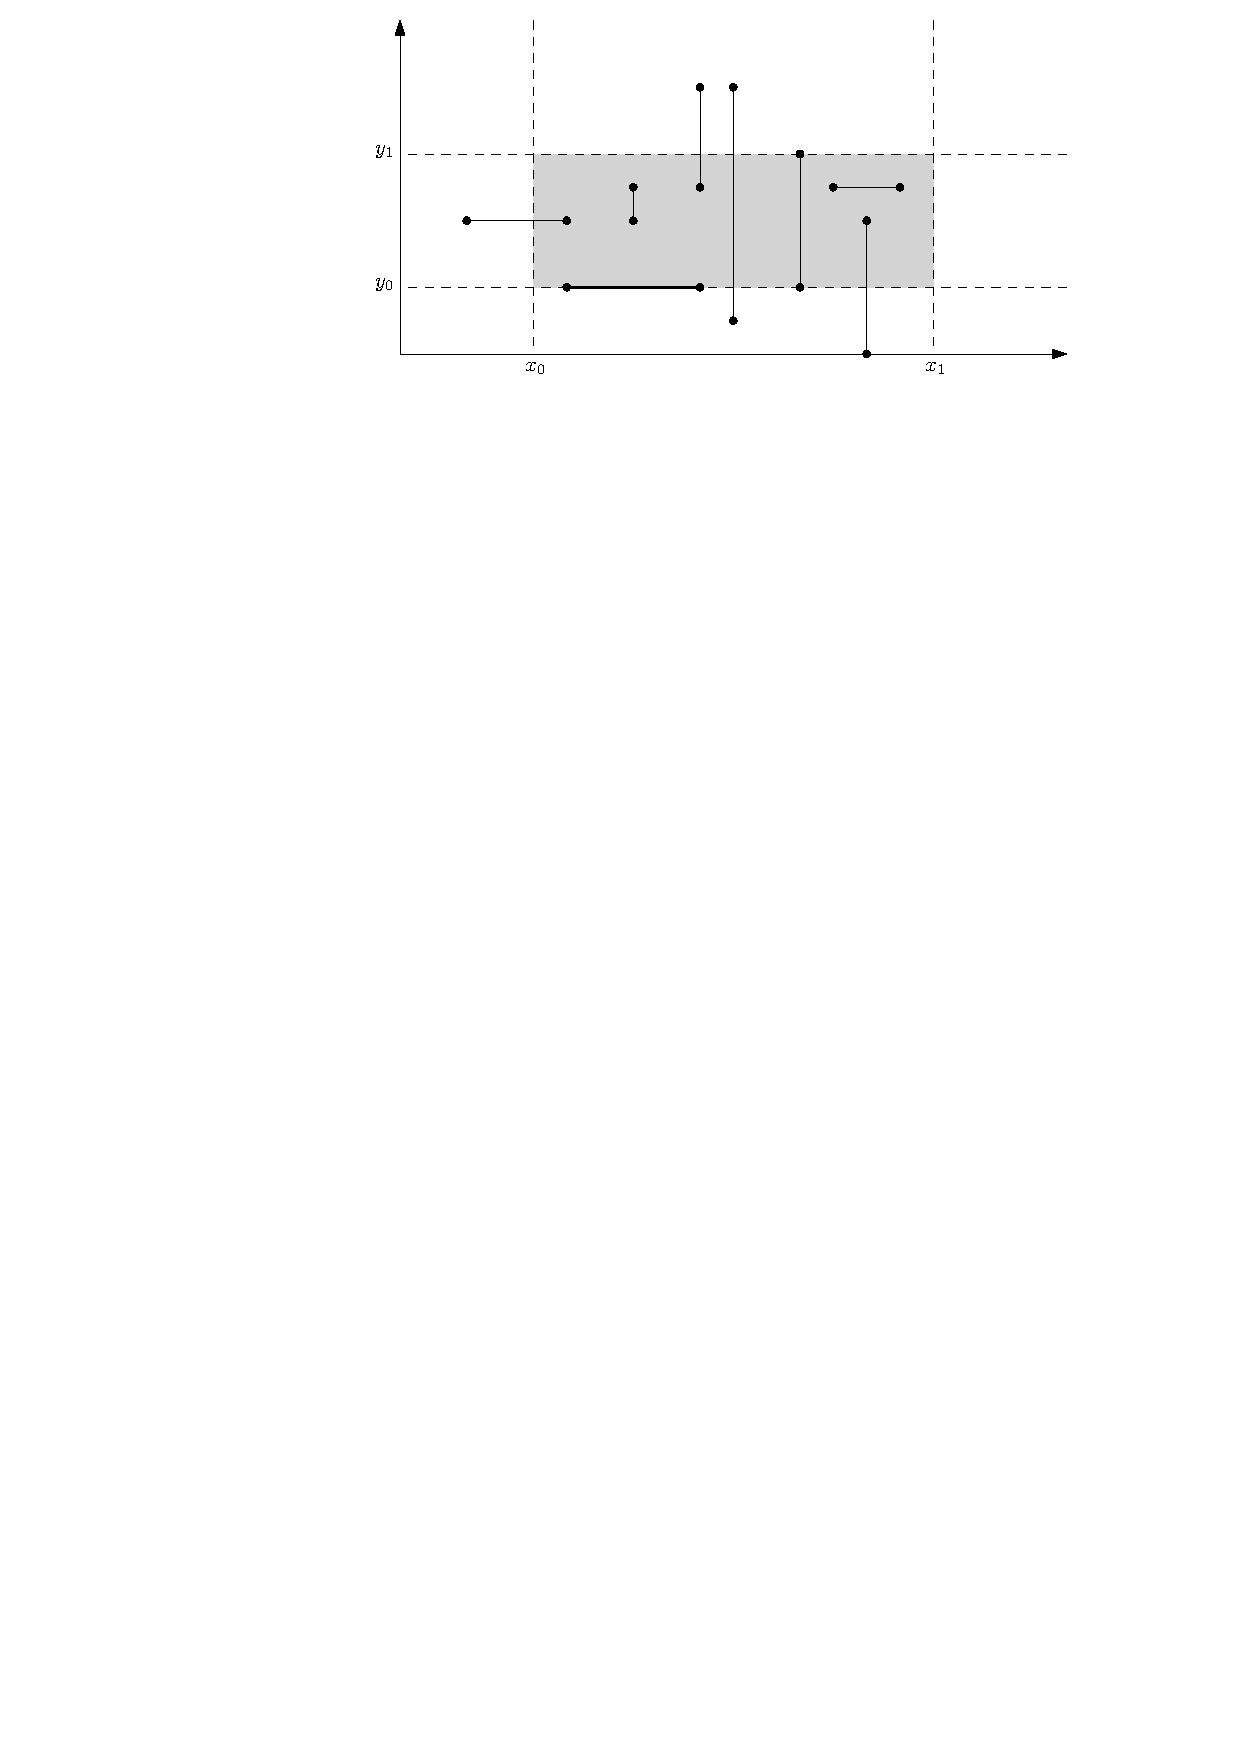
\includegraphics[scale=.8]{ipe/window-query.pdf}
\caption{Query $w = [x_0 , x_1] \times [y_0, y_1]$. }
\label{fig:stabbing-line}
\end{figure}


We can report all line segments with at least one endpoint inside $w$ using algorithms and techniques from Section \ref{sec:range-queries}. 
%
We can use 2 instances of 3-sided query i.e. $ q_0 = [x_0, x_1] \times [y_0, +\infty ]  $ and $q_1 = [x_0, x_1] \times [-\infty,y_1]$, and then report the intersections of the two queries in time $O(\log n + k_0) + O(\log n + k_1) $. 
%
However, in the worst case scenario, the two queries may report all $n = k_0 + k_1$ endpoints while the intersection may contain only one element.
%
By constructing 2D range trees with storage $O(n\log n)$, and time $O(\log^2 n + k)$ we can report all line segments with ends points in $w$. Applying fractional cascading can reduce the query time further to $O(\log n +k)$ which is faster than $(\log n + n)$.

What is left is how to handle efficiently those line segments that pass through our window query $w$? 
%
In other words, we are looking for line segments that stab two boundaries of our window query $w$.
% 
If we know how to report all line segments that stab one boundary,  say $[x_0, x_1]$, of $w$, we can easily check if they stab any of the remaining boundaries.
%
In this section, we present a data structure that can handle stabbing queries for orthogonal line segments in $O(\log n + k)$ time, and in the next section, we show how to report stabbing queries for slanted line segments in $O(\log n + k)$. 

\paragraph{Stabbing query:} Given a set of intervals $I = \{i_1, \dots, i_n\}$, and a vertical line query $\ell (x = t)$, find all intervals that are stabbed by $\ell$. 

We apply divide and conquer strategy to solve this problem. We construct recursively a balanced BST over all end points of intervals in $I$, i.e. $E_{I} = \bigcup_{[i_l, i_r] = i \in I} \{i_l, i_r\}  $.
%
While doing so, we augment this BST with extra space at each node and fill this space with appropriate intervals from $I$ as shown in Algorithm \ref{alg:build-interval}.

\begin{algorithm}[H]
    \caption{} 
    \label{alg:build-interval}
    \begin{algorithmic}[1]
        \Function{BuildInt}{$I$}
        	\State $v.val = median(E_I)$ \Comment{key stored at node $v$}
          %\If{$I $ is not empty} 
          	\State $I_{mid} \leftarrow \{ i \in I \mid i_l \leq v.val \leq i_r  \}$
          	\State $I_{left} \leftarrow \{ i \in I \mid  i_r < v.val \}$
          	\State $I_{mid} \leftarrow \{ i \in I \mid  v.val < i_l  \}$
          	\State $v.data \leftarrow I_{mid}$ \Comment{augmented data}
          	\State $v.left \leftarrow \textsc{BuildInt} (I_{left})$
          	\State $v.right \leftarrow \textsc{BuildInt} (I_{right})$ 	 
          %\EndIf
          \State return $v$.
        \EndFunction
    \end{algorithmic}
\end{algorithm}

\begin{figure}[ht!]
\centering
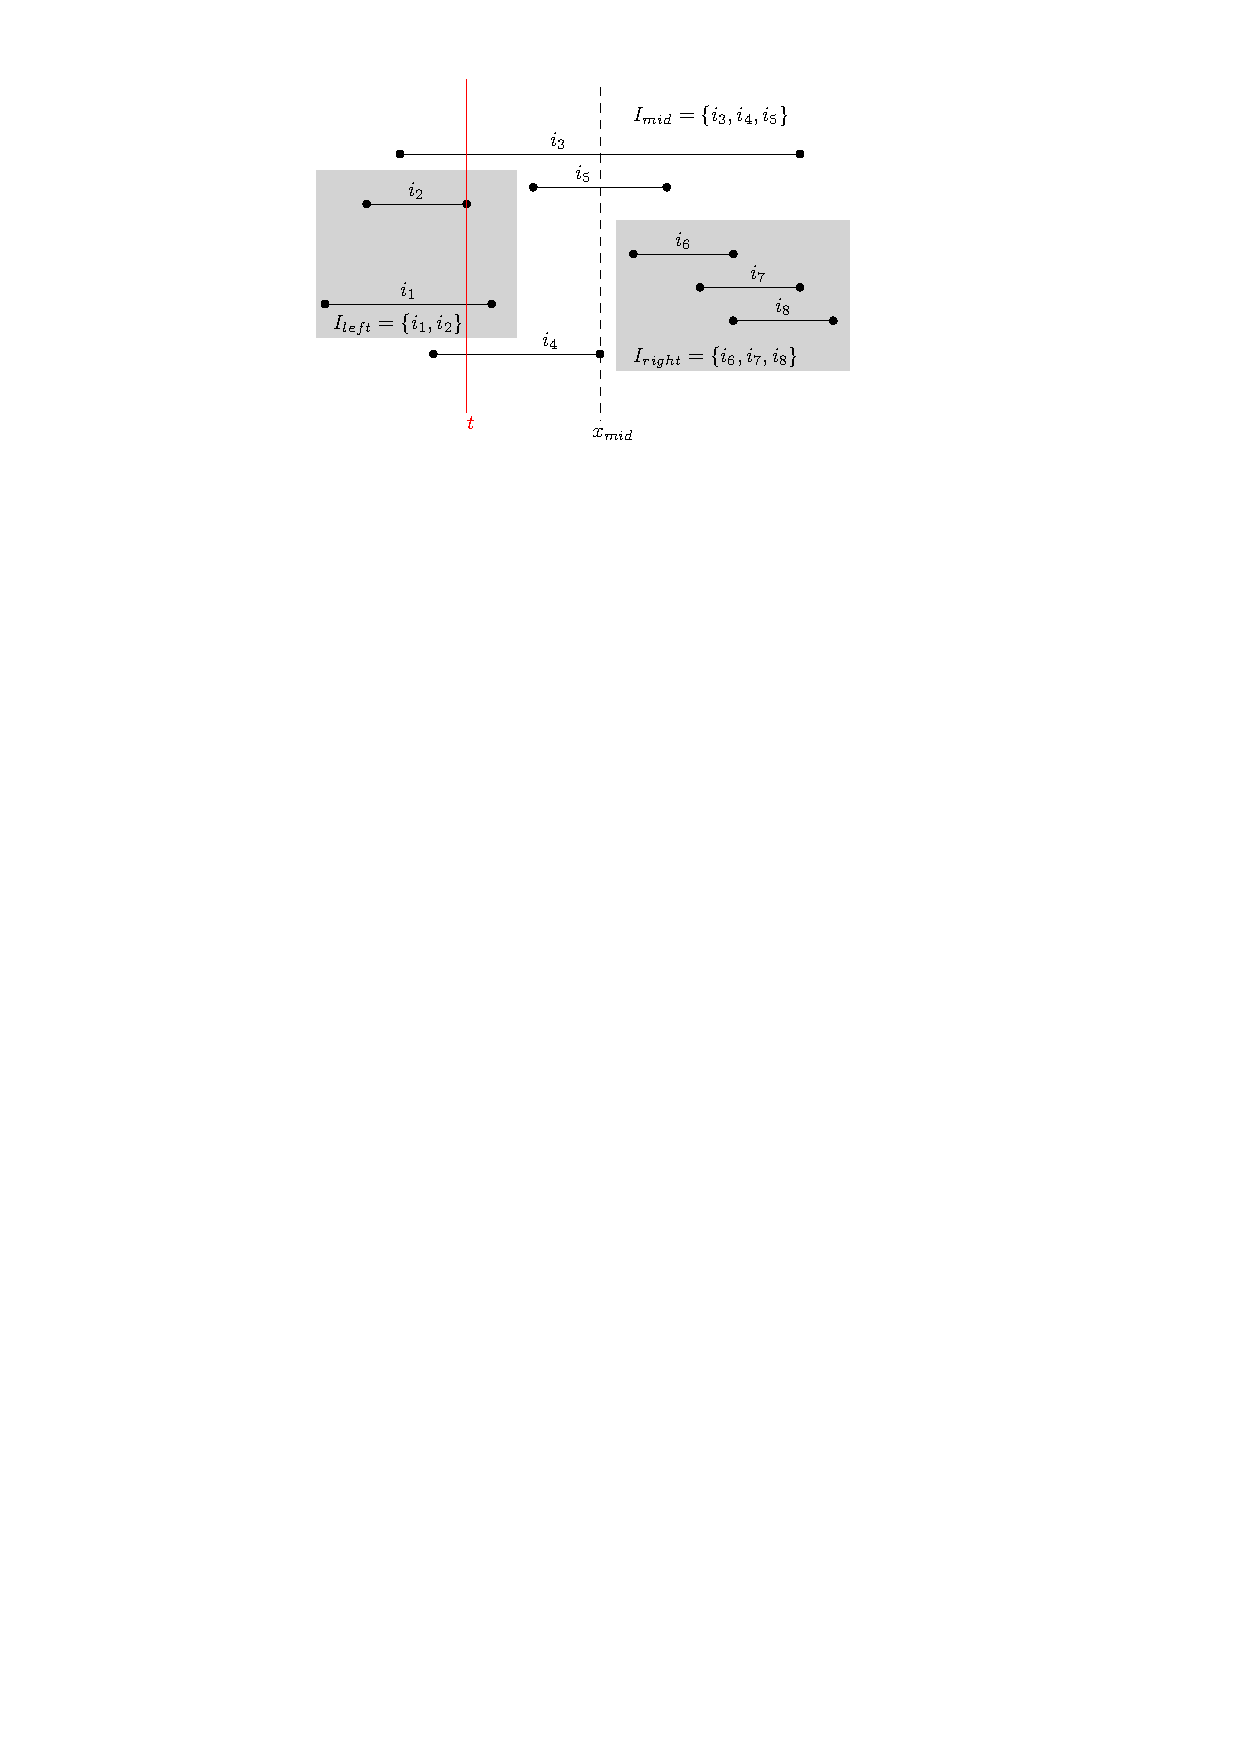
\includegraphics[scale=.8]{ipe/stabbing-line.pdf}
\caption{ $I = I_{left} \cup I_{mid} \cup I_{right} $, and $\textsc{Stab}(I, \textcolor{red}{t}) = \{ i_3, i_4, i_1, i_2 \}$.}
\label{fig:stabbing-line}
\end{figure}

Figure \ref{fig:stabbing-line} shows 8 line segments (intervals) with median being the right end point of interval $i_4$.
%
The root of the interval tree divides the set of intervals $I = \{i_1, \dots, i_8\}$ into 3 disjoint sets $I_{mid}, I_{left}, I_{right}$, where the root contains $I_{mid} = \{ i_3, i_4, i_5 \}$.
%
The left subtree will recursively store $I_{left} = \{ i_1, i_2 \}$ and the right subtree will recursively store $I_{right} =\{i_6, i_7, i_8 \}$.
% 
\paragraph{How to store $I_{mid}$?} 
In order to retrieve all intervals that are stabbed by $\textcolor{red}{q = t}$, we can scan the list of intervals stored at node $v$ for stabbed intervals before going to the left or right subtree depending on whether $\textcolor{red}{t}$ less than or greater than $v.val$.
%
However, it may happened that all $n$ intervals are stored in the root, and checking for stabbed intervals may take $O(n)$ then instead of $O(k)$, the output size!

In order to prevent that, we store $I_{mid}$ in a more efficient way by storing $I_{mid}$ sorted by the start point in an increasing order, and another copy of $I'_{mid}$ of $I_{mid}$ ordered by the end point in a decreasing order.
%
To check if $\textcolor{red}{q = t}$ stabs some intervals in $v$, we compare $\textcolor{red}{t} $ with $v.val$ and accordingly scan the list $I_{mid}$ or $I'_{mid}$ till we find an interval that does not intersect $q$.
%  
In Figure \ref{fig:stabbing-line}, at the root of the tree, $I_{mid} = \{ i_3 \leq  i_4 \leq i_5 \} $ and $I'_{mid} = \{ i_3 \geq  i_5 \geq i_4 \}$. 
%
The stabbing query would then run over $I_{mid}$ and would have $i_3 \leq i_4 \leq \textcolor{red}{t} < i_5$.  

\begin{algorithm}[H]
    \caption{} 
    \label{alg:build-interval}
    \begin{algorithmic}[1]
        \Function{QueryInt}{$v, t$}
        	\If{ $ t == v.val$ or $I_{mid} = \phi$ }
        		return $I_{mid}$
        	\EndIf
        	\If{$ t < v.val$}
        		\State return $ \{ i \in I_{mid} \mid i_l \leq t \}  \cup \textsc{QueryInt}(v.left, t)$
       		\Else 
       			\State return $\{ i \in I'{mid} \mid  i_r \geq t\} \cup \textsc{QueryInt}(v.right, t)$
        	\EndIf
          \State return $v$.
        \EndFunction
    \end{algorithmic}
\end{algorithm}

Since, we store only 2 copies of each interval $i$ in the entire tree, interval trees takes $O(n)$ space.
%
To report all stabbed intervals at node $v$, we need $k_v +1 $ comparisons. The recurrence relation is then is given by
\begin{align*} 
T(v) &= O(1 + k_v) + \max \{T(v.left) , T(v.right) \}   \\
& = O(\log n + k).
\end{align*}

The preprocessing time takes sorting complexity, as we need to build a balanced BST, sort all intervals by start point, and again by end points. 
%
We can write the recurrence relation of $\textsc{BuiltInt}$ as follows:
\begin{align*}
	T(n, h) &= O(n) + T(I_{left}, h-1) + T (I_{right}, h-1) \\
	& = O(nh) = O(n \log n).  
\end{align*}

% \subsection*{Answering the window query}
% In order to answer our original window query, we need sort $I_{mid}$ by $y$-axis  